\clearpage
\section{考察}
\begin{enumerate}[1.)]
	\item 各設定に対して,横軸が電流,縦軸が電力のグラフ(一つにまとめる)を描け.
	
	\wfig{L}に$X_{L}$での電流-電力特性を,\wfig{C}に$X_{C}$での電流-電力特性を示す.
	どちらの場合においても,力率が$1.0$に近づくほど全体的に多くの電力が得られていることがわかる.また,力率による電力への影響は電流が大きい場合であるほど大きくなっている.
	\begin{figure}[h]
	\centering
	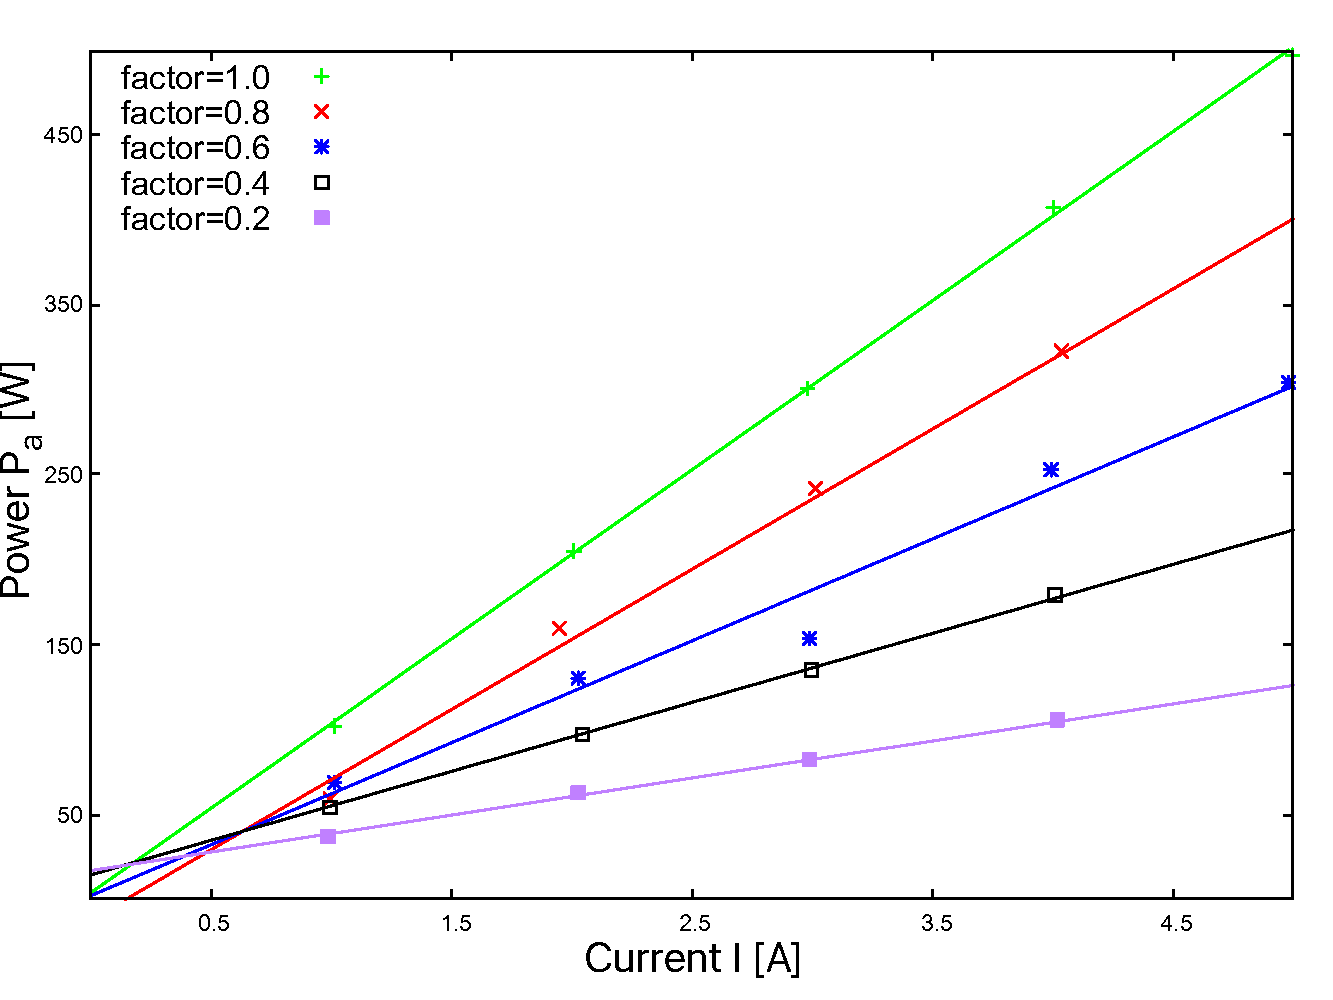
\includegraphics[scale=0.6]{./data/L/L.pdf}
	\caption{$X_L$の電流-電力特性}
	\label{fig:L}
	\end{figure}
	\begin{figure}[h]
	\centering
	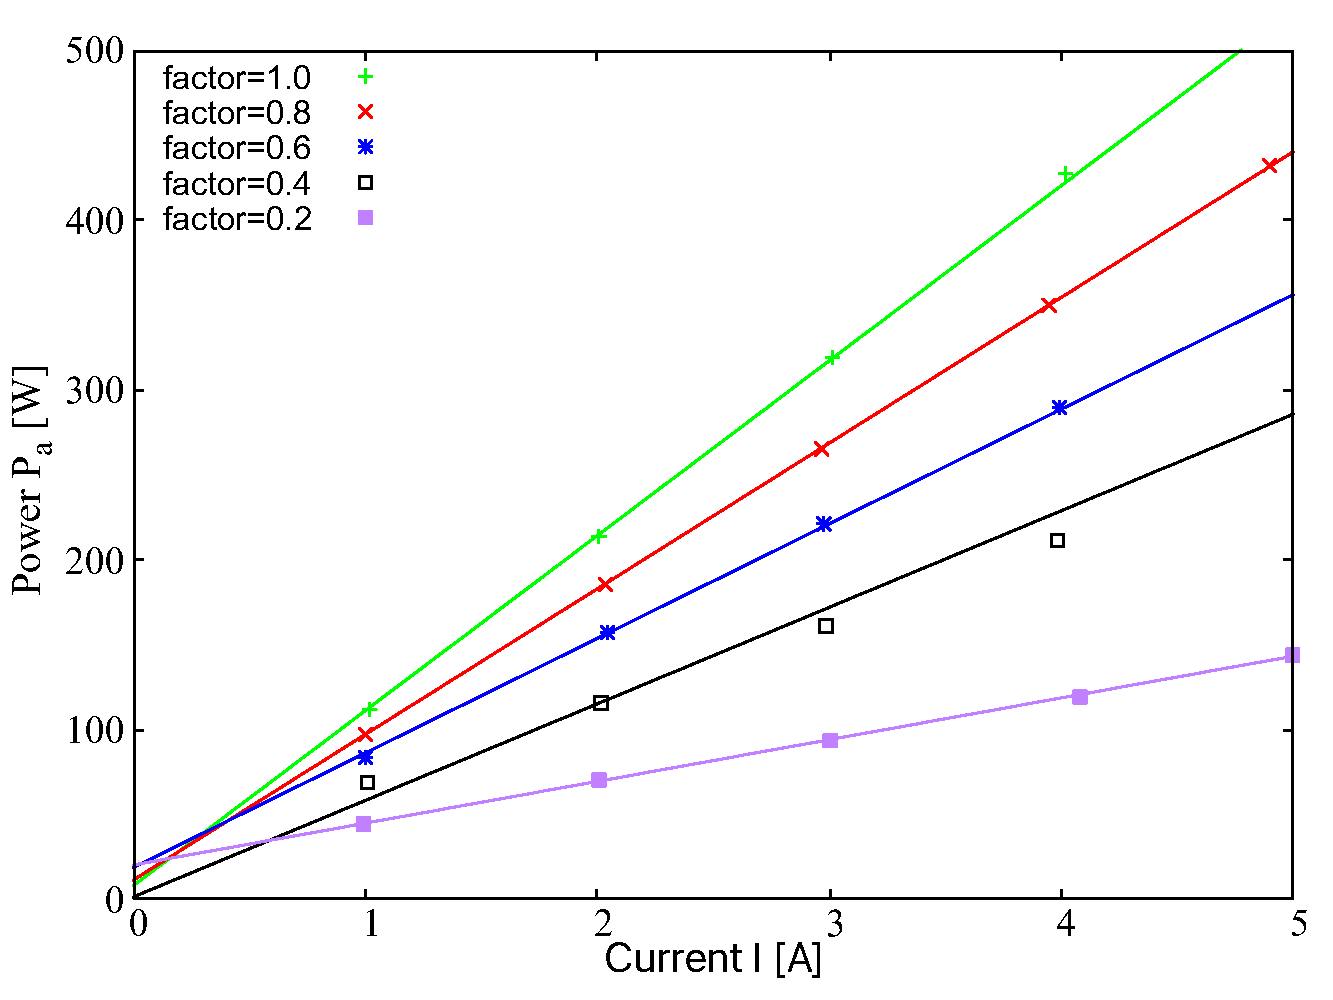
\includegraphics[scale=0.6]{./data/C/C.pdf}
	\caption{$X_C$の電流-電力特性}
	\label{fig:C}
	\end{figure}
	\item 各電流計の指示に対して,横軸が力率,縦軸が電力のグラフ(一つにまとめる)を描け.
	
	\wfig{L-fac},\wfig{C-fac}それぞれ近似直線と共に力率-電力特性を示す.
	\begin{figure}[h]
	\centering
	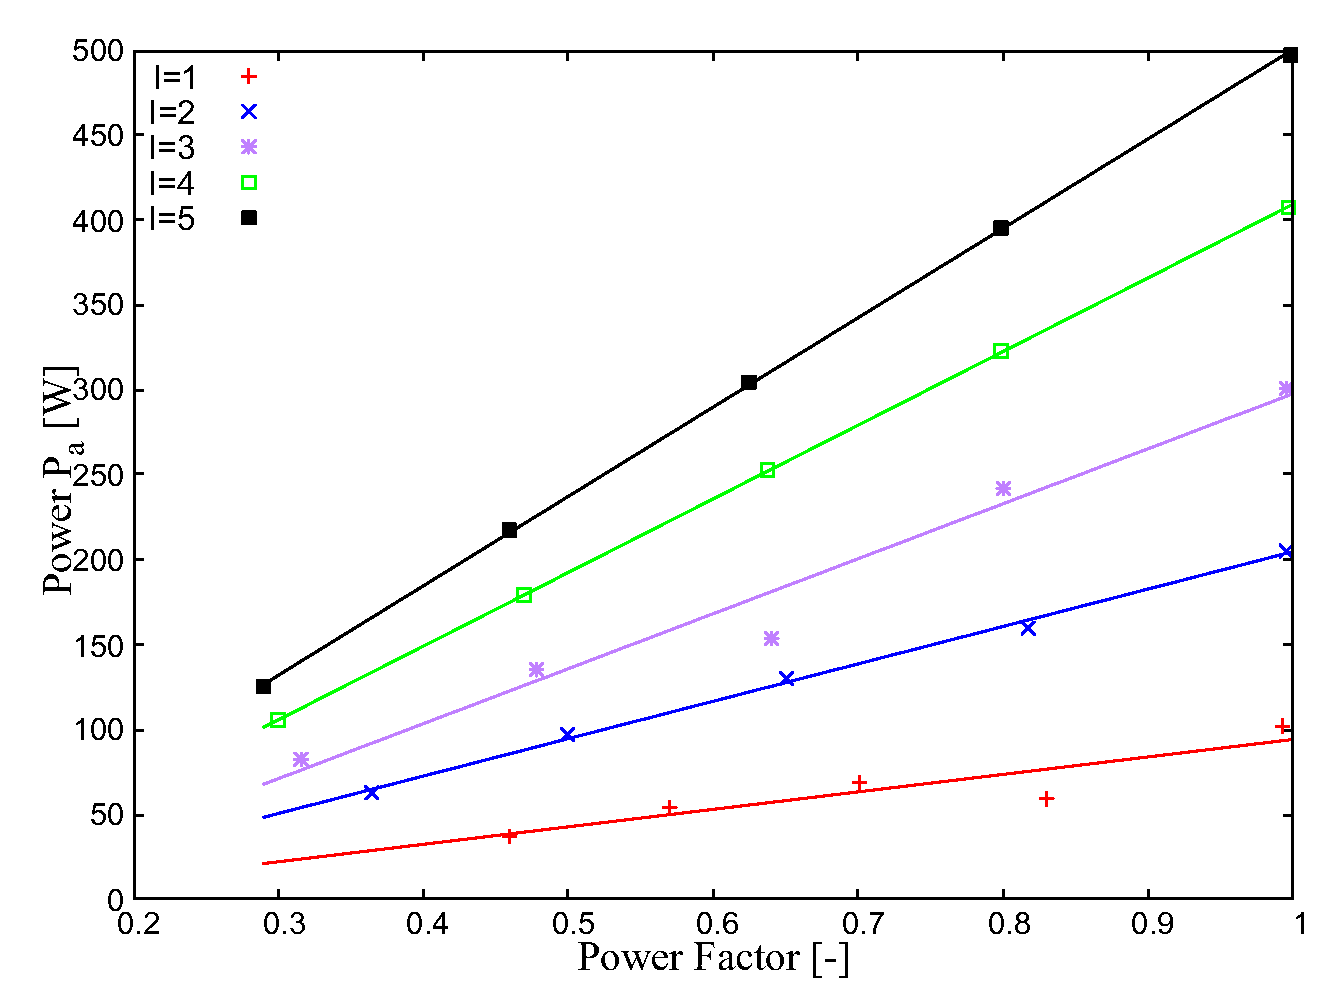
\includegraphics[scale=0.6]{./data/L/L-fac.pdf}
	\caption{$X_L$の力率-電力特性}
	\label{fig:L-fac}
	\end{figure}
	\begin{figure}[h]
	\centering
	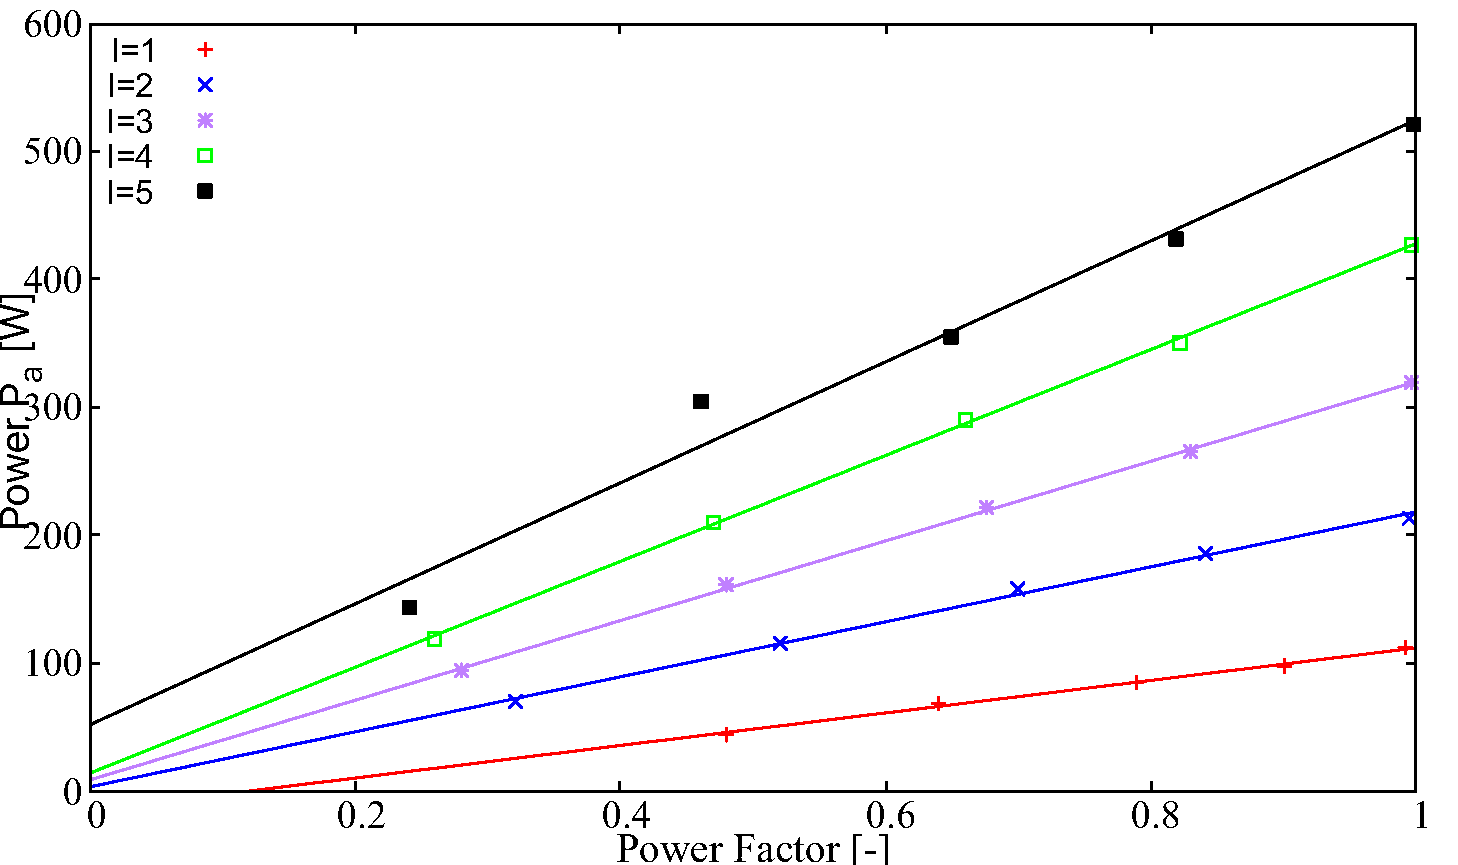
\includegraphics[scale=0.6]{./data/C/C-fac.pdf}
	\caption{$X_C$の力率-電力特性}
	\label{fig:C-fac}
	\end{figure}
	\item 電力と電圧,電流,力率の関係を述べよ.
	
	電力と電圧,電流は\weq{calpo}より比例関係にある.
	また,電力と力率も\weq{power}より比例関係にある.
	\item 普通電力計による測定結果と低力率用電力計による測定結果について比較検討せよ.
	\item グループで議論した考察を述べよ.
	\item この実験について独自の考察も加えよ.
	\item 報告書の提出〆切までに理解できなかった疑問点を挙げよ.
\end{enumerate}